% !TeX root = ../thesis.tex

\chapter{硬件实现}

\section{QEMU 模拟实现}

QEMU \cite{qemu} 为操作系统和用户态程序提供虚拟的执行环境,通过动态的二进制转换,模拟 CPU 的行为,同时支持多种外设的仿真,在系统开发中扮演着重要角色。
QEMU 支持模拟 RISC-V 运行环境,通过对 QEMU 的修改和测试,我们可以不断完善设计方案。对 QEMU 的修改主要分为四个方面:

\begin{itemize}
    \item 指令翻译:引入对 \Iuipi 指令的译码和执行;
    \item CPU 状态:维护 CSR 寄存器等 CPU 状态;
    \item 内存读写:\Iuipi 指令需要直接访问物理内存和 UINTC 外设,调用 \mintinline[breaklines]{C}{void cpu_physical_memory_rw(hwaddr addr, void *buf, hwaddr len, bool is_write)} 函数完成对物理地址的读写;
    \item 核间中断:实现 UINTC 并向各个核发送中断。
\end{itemize}

\subsection{指令翻译}

QEMU 翻译一条指令的过程为:从客户机指令(Guest Instructions)到中间码(TCG,Tiny Code Generator),最后再到宿主机指令(Host Instructions)。
QEMU 的翻译机制类似于 CPU 流水线中的译码阶段,需要定义模式串来帮助 QEMU 在执行到某一指令时调用对应的辅助函数。模式串的定义位于 target/riscv/insn32.decode :

\begin{lstlisting}
uipi_send       0000000  00000 ..... 010 ..... 1111011 @r2
uipi_read       0000001  00000 ..... 010 ..... 1111011 @r2
uipi_write      0000010  00000 ..... 010 ..... 1111011 @r2
uipi_activate   0000011  00000 ..... 010 ..... 1111011 @r2
uipi_deactivate 0000100  00000 ..... 010 ..... 1111011 @r2
\end{lstlisting}

以 \Iuret 这条指令为例,在 target/riscv/insn\_trans 目录下,有各种指令的翻译过程,主要用来将指令解析的结果(寄存器,立即数等)传递给辅助函数,将客户机指令拆解为宿主机指令来模拟目标指令的功能。
对于 \Iuret 指令的执行涉及到较多 CPU 状态的变化,会对 pc ,CSR 等产生影响, 辅助函数的定义位于 target/riscv/helper\.h,通过宏定义 DEF\_HELPER\_x 来声明辅助函数,例如:

\begin{lstlisting}[style=CStyle]
DEF_HELPER_1(uret, tl, env)
DEF_HELPER_4(csrrw, tl, env, int, tl, tl)
\end{lstlisting}

其中第一个参数对应辅助函数的名称 ,第二个参数代表函数的返回值类型(tl 表示 target\_ulong),后面的参数都是辅助函数传入的参数类型。有了以上的参考,我们可以定义其他辅助函数:

\begin{lstlisting}[style=CStyle]
DEF_HELPER_2(uipi_write, void, env, tl)
void helper_uipi_write(CPURISCVState *env, target_ulong src) {
    if (uipi_enabled(env, env->suirs)) {
        uint64_t addr = UINTC_REG_HIGH(env->suicfg, SUIRS_INDEX(env->suirs));
        cpu_physical_memory_write(addr, &src, 8);
    }
}
\end{lstlisting}

\subsection{CPU 状态维护}

CPU 状态的维护位于 target/riscv/cpu.h。这个结构同时考虑了 RV32、RV64、RV128 的情况,这些寄存器都是 CPU 运行时必要的状态。包括但不限于:

\begin{itemize}
    \item pc
    \item 整数、浮点寄存器堆
    \item CSR,有些寄存器是 M 态和 S 态复用的,例如 \Rmstatus、 \Rmip 等
    \item PMP 寄存器堆
    \item 通过 kernel\_addr、fdt\_addr 等从指定位置加载镜像
\end{itemize}

在target/riscv/cpu.h 文件末尾的表中注册 CSR 的操作函数。

中断异常、CSR 等宏定义位于 target/riscv/cpu\_bits.h ,我们需要在其中添加和 U 态有关的中断控制位。
CPU 中断异常处理函数位于 target/riscv/cpu\_helper.c 的最后,
这个函数对中断异常原因进行判断,并根据 CPU 当前的特权级做不同的处理。
这个函数只给出了 M 态和 S 态的中断异常处理,我们需要额外在此处加入委托给 U 态的中断异常处理,也就是读写 \Rustatus,\Rucause,\Ruepc 等寄存器。

\subsection{跨核中断实现}

QEMU 支持对不同硬件环境的模拟,需要在 virt 硬件环境中添加 UINTC 外设的配置并生成设备树信息。

UINTC 代码实现位于 hw/intc/riscv\_uintc.c ,调用 riscv\_uintc\_realize 对 UINTC 进行初始化,将 UINTC 外设连接到总线上,并初始化总线地址空间。对外设中的状态寄存器(接收方状态寄存器,中断信号寄存器等)进行内存分配和初始化。
通过调用 qdev\_connect\_gpio\_out 默认将 UINTC 的中断信号绑定至每个核的 \Ruip 寄存器中的 \FcsrUipUsip 位。

\begin{lstlisting}[style=CStyle]
for (i = 0; i < num_harts; i++) {
    CPUState *cpu = qemu_get_cpu(hartid_base + i);
    RISCVCPU *rvcpu = RISCV_CPU(cpu);
    qdev_connect_gpio_out(dev, i, qdev_get_gpio_in(DEVICE(rvcpu), IRQ_U_SOFT));
}
\end{lstlisting}

最后完成对 UINTC 读写函数的注册,这样就可以直接通过物理地址访问 UINTC 外设的读写端口:

\begin{lstlisting}[style=CStyle]
static const MemoryRegionOps riscv_uintc_ops = {
    .read = riscv_uintc_read,
    .write = riscv_uintc_write,
    .endianness = DEVICE_LITTLE_ENDIAN,
    .valid = {
        .min_access_size = 8,
        .max_access_size = 8
    }
};
\end{lstlisting}

在 QEMU 的 virt 硬件环境中添加设备树生成代码,生成的设备树节点内容如下:

\lstset{basicstyle=\footnotesize\tt}
\begin{lstlisting}
uintc@2f10000 {
    interrupts-extended = <0x08 0x00 0x06 0x00 0x04 0x00 0x02 0x00>;
    reg = <0x00 0x2f10000 0x00 0x4000>;
    interrupt-controller;
    compatible = "riscv,uintc0";
};
\end{lstlisting}

其中各个字段的含义为:

\begin{itemize}
    \item \textbf{interrupts-extended} 连接到每个核 \Ruip 寄存器的 \FcsrUipUsip 位;
    \item \textbf{interrupts-controller} 表示该设备是一个接收中断的控制器,这里加上是为了方便 Linux 识别,实际上 UINTC 并没有接收外部中断;
    \item \textbf{compatible} 表示设备名称,Linux 内注册驱动时应该与之对应。
\end{itemize}

在 UINTC 的实现中,中断是通过每次写入 UINTC 的端口来触发的,这和真实的硬件实现其实存在差异。
例如在 U 态,从目前的设计方案来看,需要同时满足以下几个条件才可以触发中断:

\begin{itemize}
    \item 当前特权级为 S 态;
    \item \Rustatus 中 \FcsrUstatusUie 位是 1;
    \item \Ruie 中 \FcsrUieUsie 位是 1;
    \item \Ruip 中 \FcsrUipUsip 位是 1。
\end{itemize}

在硬件实现中,可以看成是几个信号的与操作,当其他所有信号都拉高时,任何一个信号从低电平拉高都会触发中断,根据 RISC-V 的特权态规范\cite{rvpriv110},
\Isret 会将特权态从 S 态切换回 U 态,\Iuret 会将 \Rustatus 中的 \FcsrUstatusUie 位设置为 \FcsrUstatusUpie 位,在这两条指令后执行的第一条指令都有可能被中断打断并立刻进入中断处理的流程,
因此我们需要在 QEMU 中模拟这个过程,在 \Isret 和 \Iuret 指令中直接对上述条件进行判断和处理,例如在 \Isret 的辅助函数中:

\lstset{language=C}
\begin{lstlisting}[style=CStyle]
if (riscv_has_ext(env, RVN)
    && prev_priv == PRV_U
    && get_field(env->mip, MIP_USIP)
    && get_field(env->mstatus, MSTATUS_UIE)
    && get_field(env->sideleg, MIP_USIP)) {
    retpc = env->utvec;     // 直接跳转到U态中断处理入口
    env->uepc = env->sepc;  // 指定 \Iuret 到同一条指令
    mstatus = env->mstatus;
    mstatus = set_field(mstatus, MSTATUS_UPIE, 1);
    mstatus = set_field(mstatus, MSTATUS_UIE, 0);
    env->mstatus = mstatus;
}
\end{lstlisting}

\section{Rocket Chip 硬件实现}

\subsection{CPU 状态维护}

参考设计方案,在 rocket/CSR.scala 中添加读写 CSR 的逻辑,需要注意 \Ruip 等多个特权级共用的寄存器需要设置对应特权级的屏蔽位。

参考 M 态中断和异常委托的逻辑,添加 S 态委托到 U 态的逻辑,此外需要在 S 态将已委托给 U 态的中断屏蔽。

在 rocket/IDecode.scala 中添加 \Iuret 的指令解码并将指令解码注册到 \texttt{decode\_table} 中。\Iuret 的功能逻辑比较简单,只需要设置 \Rustatus 中的使能位并重新设置 pc 即可。

\begin{lstlisting}[style=CStyle,language=scala]
    // 读取 uip 寄存器
    val read_uip = read_mip & read_sideleg
    // 委托给 U 态的中断
    val delegateU = Bool(usingUser) && reg_mstatus.prv === PRV.U && delegate && read_sideleg(cause_lsbs) && cause(xLen - 1)
    // U 态的中断
    val u_interrupts = Mux(nmie && reg_mstatus.prv === PRV.U && reg_mstatus.uie, pending_interrupts & read_sideleg, UInt(0))
    // uret 的逻辑
    when (Bool(usingUser) && !io.rw.addr(9) && !io.rw.addr(8)) {
      reg_mstatus.uie := reg_mstatus.upie
      reg_mstatus.upie := true
      ret_prv := PRV.U
      io.evec := readEPC(reg_uepc)
    }
\end{lstlisting}

\subsection{UINTC 外设实现与接入}

参考 CLINT 和 PLIC 实现 UINTC 外设,首先定义 device 并指定名称和 compatible ,和 QEMU 中生成设备树的逻辑类似,在这里需要指定 UINTC 连接到 intc ,且需要指定为 interrupt-controller 让 linux 完成初始化。

\begin{lstlisting}[style=CStyle,language=scala]
    val device = new SimpleDevice("uintc", Seq("riscv,uintc0")) {
        override val alwaysExtended: Boolean = true
        override def describe(resources: ResourceBindings): Description = {
            val Description(name, mapping) = super.describe(resources)
            val extra = Map("interrupt-controller" -> Nil,
                "#interrupt-cells" -> Seq(ResourceInt(1)))
            Description(name, mapping ++ extra)
        }
    }
\end{lstlisting}

定义 node 并配置 UINTC 寄存器的读写端口,定义一系列的 \texttt{RegField} 实现读写操作,调用 \mintinline{scala}{node.regmap(opRegFields)} 进行注册:

\begin{lstlisting}[style=CStyle,language=scala]
    val node: TLRegisterNode = TLRegisterNode(
        address = Seq(params.address),
        device = device,
        beatBytes = beatBytes,
        concurrency = 1)

    // 注册 SEND 操作的写端口
    val opRegFields = uirs.zipWithIndex.flatMap { case (x, i) =>
      Seq(sendOffset(i) -> Seq(RegField(64, (),
        RegWriteFn { (valid, data) =>
            x.pending := x.pending | (valid << data(5, 0)).asUInt
            Bool(true)
        })))}
\end{lstlisting}

定义 \texttt{intnode} 连接到 CPU ,在上述 \texttt{SEND} 操作里将 \texttt{ipi} 寄存器对应位置位:

\begin{lstlisting}[style=CStyle,language=scala]
    val intnode: IntNexusNode = IntNexusNode(
        sourceFn = { _ => IntSourcePortParameters(Seq(IntSourceParameters(1,
            Seq(Resource(device, "int"))))) },
        sinkFn = { _ => IntSinkPortParameters(Seq(IntSinkParameters())) },
        outputRequiresInput = false)
    // 拉高 ipi 寄存器
    val ipi = Seq.fill(nHarts) { RegInit(0.U) }
    ipi.zipWithIndex.foreach { case (hart, i) =>
        hart := uirs.map(x => x.pending =/= 0.U && x.active && hartId(x.hartid) === i.asUInt).reduce(_ || _)
    }
    val (intnode_out, _) = intnode.out.unzip
    intnode_out.zipWithIndex.foreach { case (int, i) =>
        int(0) := ShiftRegister(ipi(i)(0), params.intStages) // usip
    }
\end{lstlisting}

将中断信号连接到对应核的 \FcsrUipUsip ,参考其他信号的处理方法,连接 \texttt{core.interrupts} 和 \texttt{intSinkNode}:

\begin{lstlisting}[style=CStyle,language=scala]
    // freechips.rocketchip.tile.SinksExternalInterrupts
    def csrIntMap: List[Int] = {
        // ...
        val usip = if (usingUser) Seq(0) else Nil
        List(65535, 3, 7, 11) ++ seip ++ usip ++ List.tabulate(nlips)(_ + 16)
    }
    // freechips.rocketchip.subsystem.CanAttachTile
    // 将 intSinkNode 的输入连接到 Rocket 处理器
    def decodeCoreInterrupts(core: TileInterrupts): Unit = {
        // ...
        val usip = if (core.usip.isDefined) Seq(core.usip.get) else Nil
        // ...
        val (interrupts, _) = intSinkNode.in(0)
        (async_ips ++ periph_ips ++ seip ++ usip ++ core_ips).zip(interrupts).foreach { case(c, i) => c := i }
    }
\end{lstlisting}

\subsection{UIPI 协处理器实现}

UIPI 协处理器负责处理自定义 \Iuipi 指令,基于 RoCC 实现,应用 RoCC 的访存端口处理 \Iuipi 指令涉及的访存请求。

RoCC 位于流水线的写回阶段,读写 CSR 时需要考虑写后读冲突,RoCC 读 \Rsuirs 和 \Rsuist 寄存器时需要增加前传逻辑。

\begin{lstlisting}[style=CStyle,language=scala]
    // 前传逻辑,以 suirs 寄存器为例
    when (decoded_addr(CSRs.suirs)) {
        val new_suirs = new SUIRS().fromBits(wdata)
        reg_suirs := new_suirs
        io.uintr.suirs := new_suirs
    }.otherwise {
        io.uintr.suirs := reg_suirs
    }
\end{lstlisting}

根据 Rocket Chip 的配置方法,在 Tile 中添加 UIPI 协处理器:

\begin{lstlisting}[style=CStyle,language=scala]
    class WithUIPI extends Config((_, _, _) => {
        case BuildRoCC => Seq((p: Parameters) => {
            // 指定该 RoCC 处理符合 OpcodeSet.custom3 格式的指令
            val module = LazyModule(new UIPI(OpcodeSet.custom3)(p))
            module
        })
    })
\end{lstlisting}

UIPI 协处理器接收译码结果并根据操作码来执行不同处理流程,状态机各个状态描述如下:

\begin{itemize}
    \item \texttt{\textbf{s\_idle}} 默认状态,等待接收处理器传来的操作请求;
    \item \texttt{\textbf{s\_wait\_mem0}} \Iuipisend 指令发起读内存请求并等待响应;
    \item \texttt{\textbf{s\_read\_uist}} \Iuipisend 指令处理响应并根据返回数据计算出访问 UINTC 的地址,根据数据缓存的 \texttt{s2\_nack} 信号判断是否需要重新发起请求;
    \item \texttt{\textbf{s\_wait\_mem1}} 发起读或写 UINTC 请求并等待响应;
    \item \texttt{\textbf{s\_check\_nack0}} 等待数据缓存响应;
    \item \texttt{\textbf{s\_check\_nack1}} 根据数据缓存的 \texttt{s2\_nack} 信号判断是否需要重新发起请求;
    \item \texttt{\textbf{s\_resp}} 响应处理器请求,\Iuipiread 需要返回写入目标寄存器的内容;
    \item \texttt{\textbf{s\_error}} 指令格式错误、访存错误、权限错误、发送方状态表项错误。
\end{itemize}

\begin{figure}
    \centering
    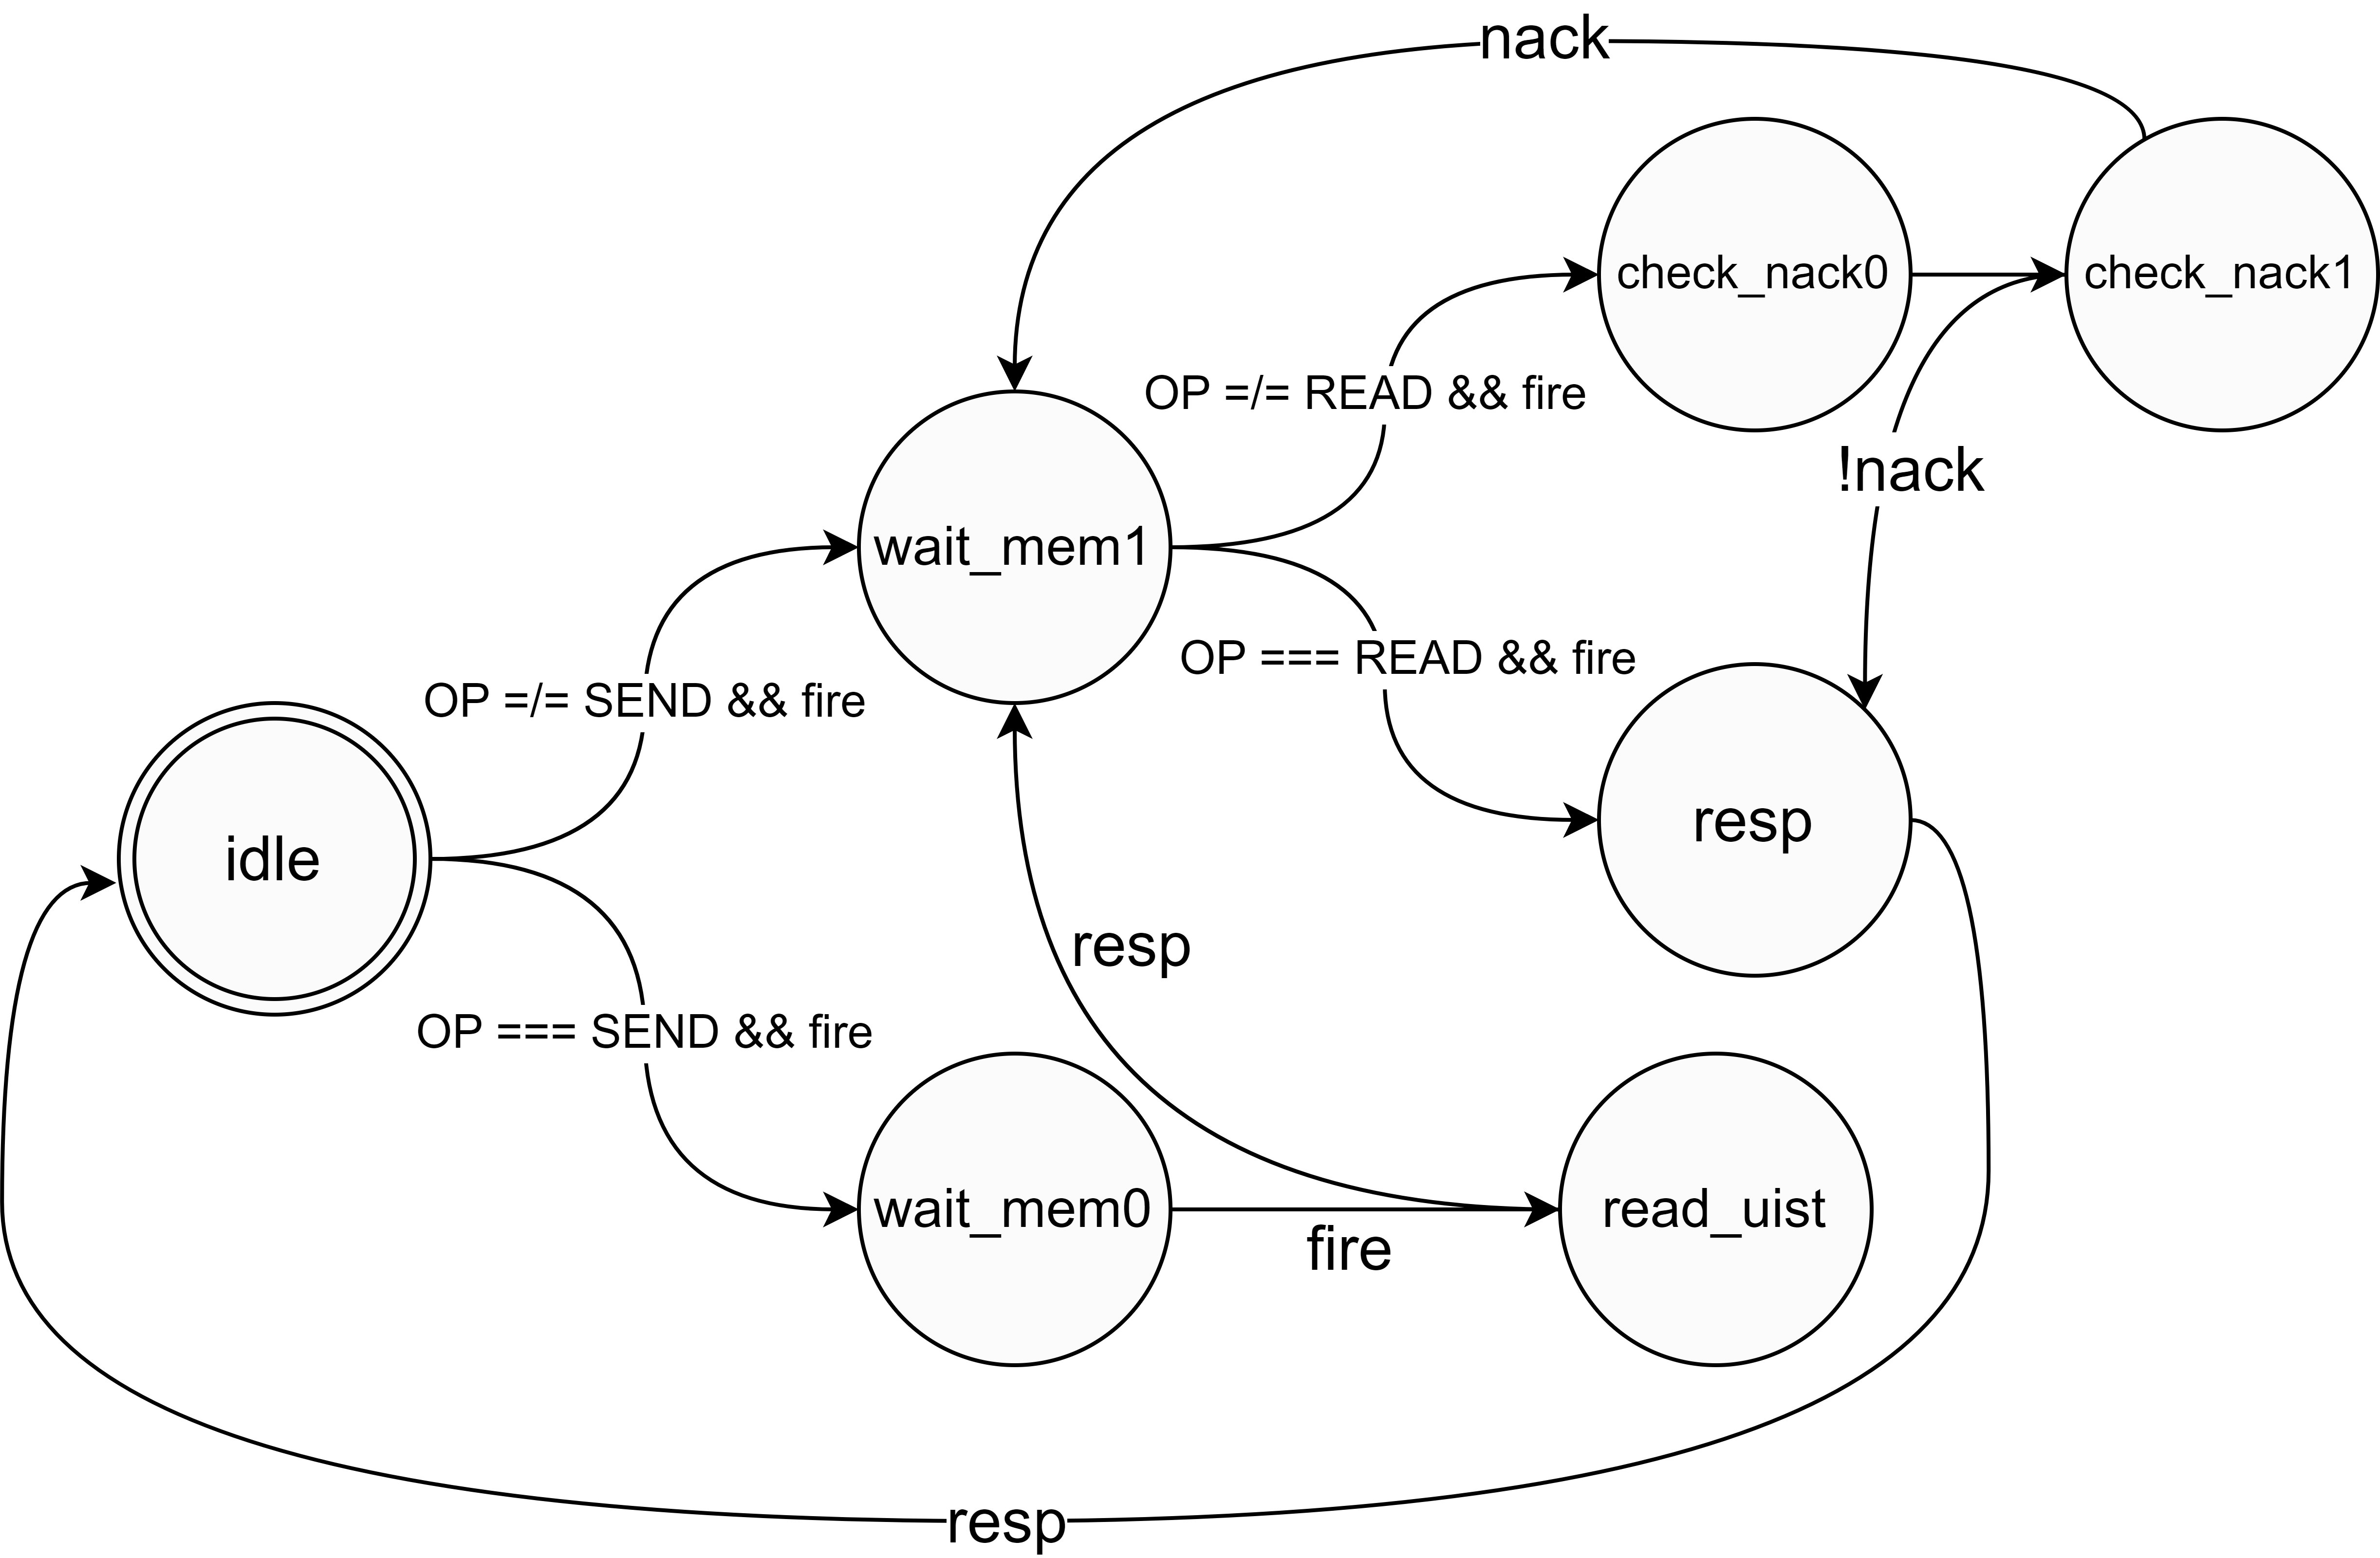
\includegraphics[width=0.8\linewidth]{figures/uintr3.png}
    \caption{UIPI 协处理器工作流程}
    \label{fig:uintr3}
\end{figure}

UIPI 协处理器共发出三类访存请求:读内存,读外设,写外设,其中读内存请求可能因为数据缓存不命中需要重新发起请求,读写外设请求可能因为数据缓存事务繁忙需要重新发起请求,因此在处理流程中加入了对数据缓存 \texttt{s2\_nack} 信号的处理。此外,在 Rocket Chip 中存在一个缓存多个 RoCC 读写请求的队列模块,支持失败读写请求的重试,然而对于写外设请求,队列会持续等待响应信号并阻塞。因为目前只有一个 UIPI 协处理器,所以在架构中移除了这个模块并直接将 UIPI 协处理器连接到数据缓存的仲裁器。
